
表达式求值要解决的问题一般是输入一个字符串表示的表达式,要求输出它的值。当然也有变种比如表达式中是否包含括号,指数运算,含多少变量,判断多个表达式是否等价,等等。

其中判断表达式等价的部分使用了拉格朗日插值法等数学工具,在此暂不进行展开。

一般的思路分为两种,一种递归一种非递归。

\subsection{递归}

递归的方法是把表达式拆分成如图所示的表达式树,然后在树结构上自底向上进行运算。

\begin{figure}[htbp]
\centering
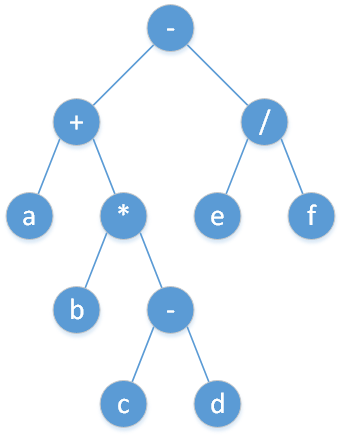
\includegraphics[width=0.7\textwidth]{docs/basic/images/bet.png} 

\end{figure}

表达式树上进行  树的遍历  可以得到不同类型的表达式

\begin{itemize}
\item 前序遍历对应前缀表达式(波兰式)
\item 中序遍历对应中缀表达式
\item 后序遍历对应后缀表达式(逆波兰式)
\end{itemize}

\subsection{非递归}

非递归的方法是定义两个  栈  来分别存储运算符和运算数。每当遇到一个数直接放进数的栈;每当遇到一个操作符时,要查找之前运算符栈中的元素,按照预先定义好的优先级来进行适当的弹出操作(弹出的同时求出对应的子表达式的值)。

我们要知道:算术表达式分为三种,分别是前缀表达式、中缀表达式、后缀表达式。其中,中缀表达式是我们日常生活中最常用的表达式;后缀表达式是计算机最容易理解的表达式。为什么说后缀表达式最容易被计算机理解呢?因为后缀表达式不需要括号表示,它的运算顺序是唯一确定的。举个例子:在后缀表达式 $3 2 * 1 -$ 中,首先计算 $3 \times 2 = 6$(使用最后一个运算符,即栈顶运算符),然后计算 $6 - 1 = 5$。可以看到:对于一个后缀表达式,只需要 \textbf{ 维护一个数字栈,每次遇到一个运算符,就取出两个栈顶元素,将运算结果重新压入栈中 }。最后,栈中唯一一个元素就是改后缀表达式的运算结果时间复杂度 $O(n)$。

所以说,对于普通中缀表达式的计算,我们可以将其转化为后缀表达式再进行计算。转换方法也十分简单。只要建立一个用于存放运算符的栈,扫描该中缀表达式:

\begin{enumerate}
\item 如果遇到数字,直接将该数字输出到后缀表达式(以下部分用「输出」表示输出到后缀表达式)
\item 如果遇到左括号,入栈
\item 如果遇到右括号,不断输出栈顶元素,直至遇到左括号。(左括号出栈,但不输出)
\item 如果遇到其他运算符,不断去除所有运算优先级大于等于当前运算符的运算符,输出。最后,新的符号入栈。
\item 把栈中剩下的符号依次输出,表达式转换结束。
\end{enumerate}

时间复杂度 $O(n)$.

示例代码:

\begin{cppcode}
// 下面代码摘自笔者 NOIP2005 等价表达式
std::string convert(const std::string &s) {  // 把中缀表达式转换为后缀表达式
  std::stack<char> oper;
  std::stringstream ss;
  ss << s;
  std::string t, tmp;
  while (ss >> tmp) {
    if (isdigit(tmp[0]))
      t += tmp + " ";  // 1. 如果遇到一个数,输出该数
    else if (tmp[0] == '(')
      oper.push(tmp[0]);       // 2. 如果遇到左括号,把左括号入栈
    else if (tmp[0] == ')') {  // 3. 如果遇到右括号,
      while (!oper.empty() && oper.top() != '(')
        t += std::string(1, oper.top()) + " ",
            oper.pop();  // 不断取出栈顶并输出,直到栈顶为左括号,
      oper.pop();        // 然后把左括号出栈
    } else {             // 4. 如果遇到运算符
      while (!oper.empty() && level[oper.top()] >= level[tmp[0]])
        t += std::string(1, oper.top()) + " ",
            oper.pop();  // 只要栈顶符号的优先级不低于新符号,就不断取出栈顶并输出
      oper.push(tmp[0]);  // 最后把新符号进栈
    }
  }
  while (!oper.empty()) t += std::string(1, oper.top()) + " ", oper.pop();
  return t;
}

int calc(const std::string &s) {  // 计算转换好的后缀表达式
  std::stack<int> num;
  std::stringstream ss;
  ss << s;
  std::string t, tmp;
  while (ss >> tmp) {
    if (isdigit(tmp[0]))
      num.push(stoi(tmp));
    else {
      int b, a;  // 取出栈顶元素,注意顺序
      if (!num.empty()) b = num.top();
      num.pop();
      if (!num.empty()) a = num.top();
      num.pop();
      if (tmp[0] == '+') num.push(a + b);
      if (tmp[0] == '-') num.push(a - b);
      if (tmp[0] == '*') num.push(a * b);
      if (tmp[0] == '^') num.push(qpow(a, b));
    }
  }
  return num.top();
}
\end{cppcode}

\subsection{习题}

\begin{enumerate}
\item \href{https://www.luogu.org/problemnew/show/P1981}{表达式求值 (NOIP2013)}
\item \href{https://www.luogu.org/problemnew/show/P1449}{后缀表达式}
\item \href{https://www.spoj.com/problems/ONP/}{Transform the Expression}
\end{enumerate}
